\chapter{Introduction}
\label{sec:introduction}

\subsection{Motivation}
\label{sec:motivation}

\todo{lots of ``systems'' written here}

Modern physical systems, particularly those associated with public use such as freeway networks and water supplies, exist within a world with decreasing physical space and resources. For instance, freeways often cannot add additional lanes to accommodate increased demands. Thus, one must rely upon better managament systems and control algorithms in order to maximize performance within the limitations of the existing system. These ``smart'' systems make use of sensing instrumentation to estimate real-time conditions and modeling of the underlying physical dynamics to predict and plan for future states.

The focus of this thesis is the development of methods for the intelligent modeling and control of such networked dynamical systems. The goal is to provide operational managers with scalable, flexible, and robust algorithms that can leverage the well-instrumented and highly-connected control infrastructure present on modern systems. 

The remainder of this section discusses the \emph{Connected Corridors} project (Section~\ref{sec:connected-corridors}) on integrated freeway-corridor management (ICM), which served as the context in which this work was conducted, followed by an overview of \emph{model predictive control} (MPC) methods and their suitability in solving some of the main objectives put forth in the \emph{Connected Corridors} project (Section~\ref{sec:model-predictive-control}). The section concludes with a summary of the original contributions presented in this thesis (Section~\ref{sec:contributions}).

\subsection{Connected Corridors}
\label{sec:connected-corridors}

\emph{Connected-Corridors} is a project funded by the California Department of Transportation with the goal of creating the next generation of traffic management tools~\cite{connected-corridors,miller2010san}. While most current systems consider the freeway networks as independent from the city-street \emph{arterial} road networks, \emph{Connected Corridors} is tasked with creating an integrated approach to traffic management (referred to as ICM) which accounts for their dual performance. The project has demonstrated innovative control and estimation approaches to ICM on macroscopic and microscopic simulation environments (presented in Section~\ref{sec:numerical-results-adjoint}), with the ultimate plan of transferring the knowledge to a physical test-site within California.

The proposed ICM system possesses the following capabilities.

\begin{itemize}
	\item \textbf{Estimation}: Operators have access to a real-time estimation of the traffic conditions along the major freeways and adjacent arterials.
	\item \textbf{Simulation}: Well-calibrated and efficient traffic models allow operators to simulate many different future traffic conditions.
	\item \textbf{Control}: Traffic signal and message sign plans are computed online for many specialized objectives and serve as an optimized decision support tool~\cite{Reilly2013b,Reilly2014b}.
\end{itemize}

Control schemes implemented by the system include coordinated traffic light metering plans on freeway onramps (commonly referred as ramp metering, see Section~\ref{sec:continous-and-discrete-traffic-model-for-ramp-metering}) and traffic flow diversion around incidents via changeable message signs~\cite{Samaranayake2014}. 

\begin{figure}[htbp]
	\centering
	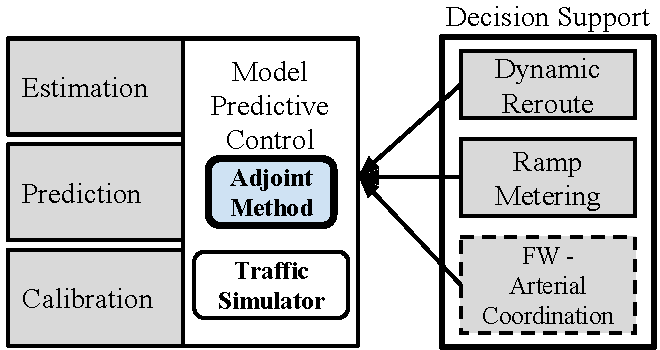
\includegraphics[width=0.8\textwidth]{diagrams/f2}
	\caption{\emph{Connected Corridors} control system architecture. The freeway state estimation, prediction and calibration submodules enable an MPC-based framework that computes coordinated, predictive decision-support strategies for numerous applications. Limited customization is required to extend the adjoint-based MPC controller to specific objectives or actuation types.}
	\label{fig:decision-support}
\end{figure}

To satisfy the above requirements, \emph{Connected Corridors} focuses on a number of submodules which are developed independently, but composed arbitrarily to create high-level, comprehensive support tools. Figure~\ref{fig:decision-support} shows a diagram of the several of the developed submodules and how they can be composed to create an MPC controller (explained in Section~\ref{sec:model-predictive-control}). Subsequently, the controller submodule is leveraged by a number of actuation strategies which have similar architectural requirements. For instance, both ramp metering and dynamic rerouting require real-time estimation and a calibrated freeway model to compute effective control strategies. Via submodule composition, much of the technology can be reused between the applications.

\subsection{Model Predictive Control}
\label{sec:model-predictive-control}

\begin{itemize}
	\item how it fits within CC project
	\item how it can be exploited by attackers
\end{itemize}

\subsection{Contributions}
\label{sec:contributions}